\documentclass{scrartcl}

\usepackage{amssymb}
\usepackage{amsmath}
\usepackage{tikz}

\begin{document}
	
	%\begin{figure}
	%	\centering
	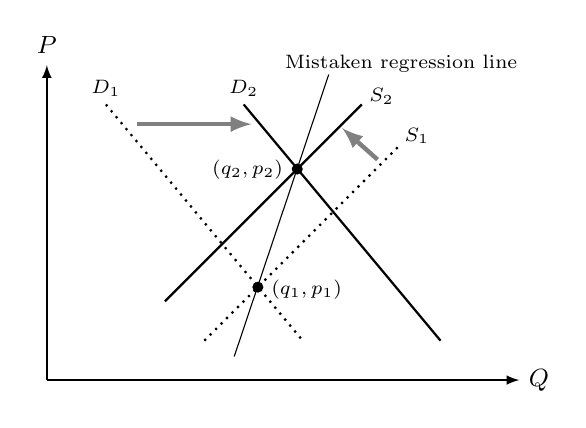
\begin{tikzpicture}
	\draw[->,>=latex,semithick] (0,0)--(0,4);
	\draw[->,>=latex,semithick] (0,0)--(6,0);
	\node at (0,4.25) {{\small $P$}};
	\node at (6.25,0) {{\small $Q$}};
	
	%demand curves
	\draw[thick,dotted] (0.75,3.5)--(3.25,0.5);
	\draw[thick] (2.5,3.5)--(5,0.5);
		\node at (0.75,3.7) {{\scriptsize $D_1$}};
		\node at (2.5,3.7) {{\scriptsize $D_2$}};
	\draw[->,>=latex,ultra thick,gray] (1.15,3.25)--(2.6,3.25);	%arrow from D1 to D2
	
	%supply curves
	\draw[thick,dotted] (2,0.5)--(4.5,3);
	\draw[thick] (1.5,1)--(4,3.5);
		\node at (4.7,3.1) {{\scriptsize $S_1$}};
		\node at (4.25,3.6) {{\scriptsize $S_2$}};
	\draw[->,>=latex,ultra thick,gray] (4.2,2.8)--(3.75,3.2);	%arrow from S1 to S2
	
	%regression line
	\fill (3.18,2.68) circle (2pt);	%upper intersection
	\fill (2.68,1.18) circle (2pt);	%lower intersection
		\node at (3.3,1.15) {{\scriptsize $(q_1,p_1)$}};
		\node at (2.55,2.67) {{\scriptsize $(q_2,p_2)$}};
	\draw (2.38,0.3)--(3.58,3.88);
		\node at (4.5,4.02) {{\scriptsize Mistaken regression line}};
	
	%\draw[help lines] (0,0) grid (6,4);
	\end{tikzpicture}
	%	\caption{Identification problem: shift in both supply and demand}
	%\end{figure}
	
\end{document}